\chapter{Model Deployments} \label{chap:deployment}
Deploying machine learning model is integrating a machine learning model to existing or new product to enable end users to benefit from it.
Although it ofter overlooked deployment is the most important part of the machine learning which without it artifacts only sits in a machine and occupy storage space.
Only by deploying models, machine learning can create a value to solve a specific problem.
One of the reasons behind deployments being neglected is the complexities surrounding the deployment process.
These difficulties includes the data collection, dependency management, feature engineering, versioning and etc.
Another difficulty is choosing the right deployment method for the problem.
Most popular ones among these large possibility of choices are maintaining a server to serve any prediction request or utilize serverless infrastructure serve prediction as they arrive.
However the options for deploying models have exploded in recent times with the increase in demand for the intelligent systems.
For this project I have chosen to use a relatively new deployment option by serving the model via static website.
Serving the model this way is only possible because of the rich ecosystem of the TensorFlow~\cite{tensorflow}.
Deployment relies on the JavaScript language and the specific framework called TensorFlow.js~\cite{tensorjs} to retrieve the model file and enable users input to make predictions on that model.
Static website that host the model in this project is currently online and accessible via the url~\footnote{https://bbuluttekin.github.io/MSc-Project/} of the website.

\section{Why this deployment choice} \label{sec:whythisdeploy}
Main reasons behind the decision of deploying machine learning model via static webpage is two fold.
First and most important reason is the financial cost of maintain the model deployment.
From the beginning, I wanted this project to be zero cost model to demonstrate that similar project that aims at social good and non-profit initiatives can achieve and maintain their goal with a limited resources.
This attribute also enables me to maintain the deployment for a very long time.
In fact, I am not planning to disconnect it in foreseeable future. 
Secondary reason is the transparency that comes from this deployment method.
Deploying as a static webpage means that the user can see and read the source code of the page and explore which model makes the prediction and how it makes it.

\section{Critical evaluation of the deployment model}
Every deployment type has a strengths and weaknesses when compare to the other available choices.
Therefore, it is imperative for me to discuss the pros and cons associated with the static website based deployments.
I have previous mentioned some of the qualities that made this deployment model attractive in the previous section, however for the interest of full disclosure I have also listed them below.
These qualities are:

\begin{itemize}
    \item Very little or no cost of deployment.
    \item Deployment details are transparent
    \item Privacy, user data does not leave the users computer
\end{itemize}

First two item in this list explained in section \ref{sec:whythisdeploy}, but it is also important to touch on last item which is the privacy element of this deployment.
Static website deployment works by bringing machine learning model to users browser and does not require connection to third party server to receive the data.
This will imply that the user data does not leave the users browser and their privacy is protected along with their data.

As oppose to these positive attributes there are some downsides to deploying machine learning model with this method.
Some of these downsides are:

\begin{itemize}
    \item Model is available to anyone for downloading
    \item Loading the model takes longer than other methods
\end{itemize}

There is no doubt that the transparency for user to inspecting the model comes with a challenge for the companies or profit driven initiatives about protecting the propriety software.
Anybody that have an access to website can download and use the trained model for themselves.
This issue becomes more apparent when considering that even competitors of an enterprise can access and used model for their on benefit.
Considering all above, this deployment model is not a good option for models that contain intellectual property.
Another downside of this deployment is that it's reliance on resource of the user.
Very complex machine learning models have millions to billions parameters with many layers that contain them.
All this complexity translates into bigger and bigger sized models that needs to be deployed. 
Considering model size for this project is around 200 to 600 MB
implies there is a need for wait for user browser to load the entire model.
Waiting time on this step can vary depending on the users internet connection speed.
This poses a significant challenge because most users would be unwilling to wait if they are not motivated to use the website.
If the project is not important to user this deployment option should be reconsidered by the developer.

\section{Implementation steps}
Implementation of this deployment can be broken down to three step.

\begin{itemize}
    \item Converting the saved model to applicable format 
    \item Creating HTML file that will be served to users 
    \item Building JavaScript file for user interactions
\end{itemize}

Model conversion step is the easiest step among other steps.
Converting TensorFlow or Keras model to compatible format is provided by TensorFlow as a command line tool and a straightforward process that can be completed at the start.
Typical scenario for the usage of this model includes, user visiting the website, user choosing and loading the image they would like to get predictions and finally clicking prediction button to receive the relevant prediction.
Considering the scenario above HTML file is created with the input field, predict button, instructions and the spinner to inform user that model loading process is initiated.

\begin{figure}[H]
    \centering
    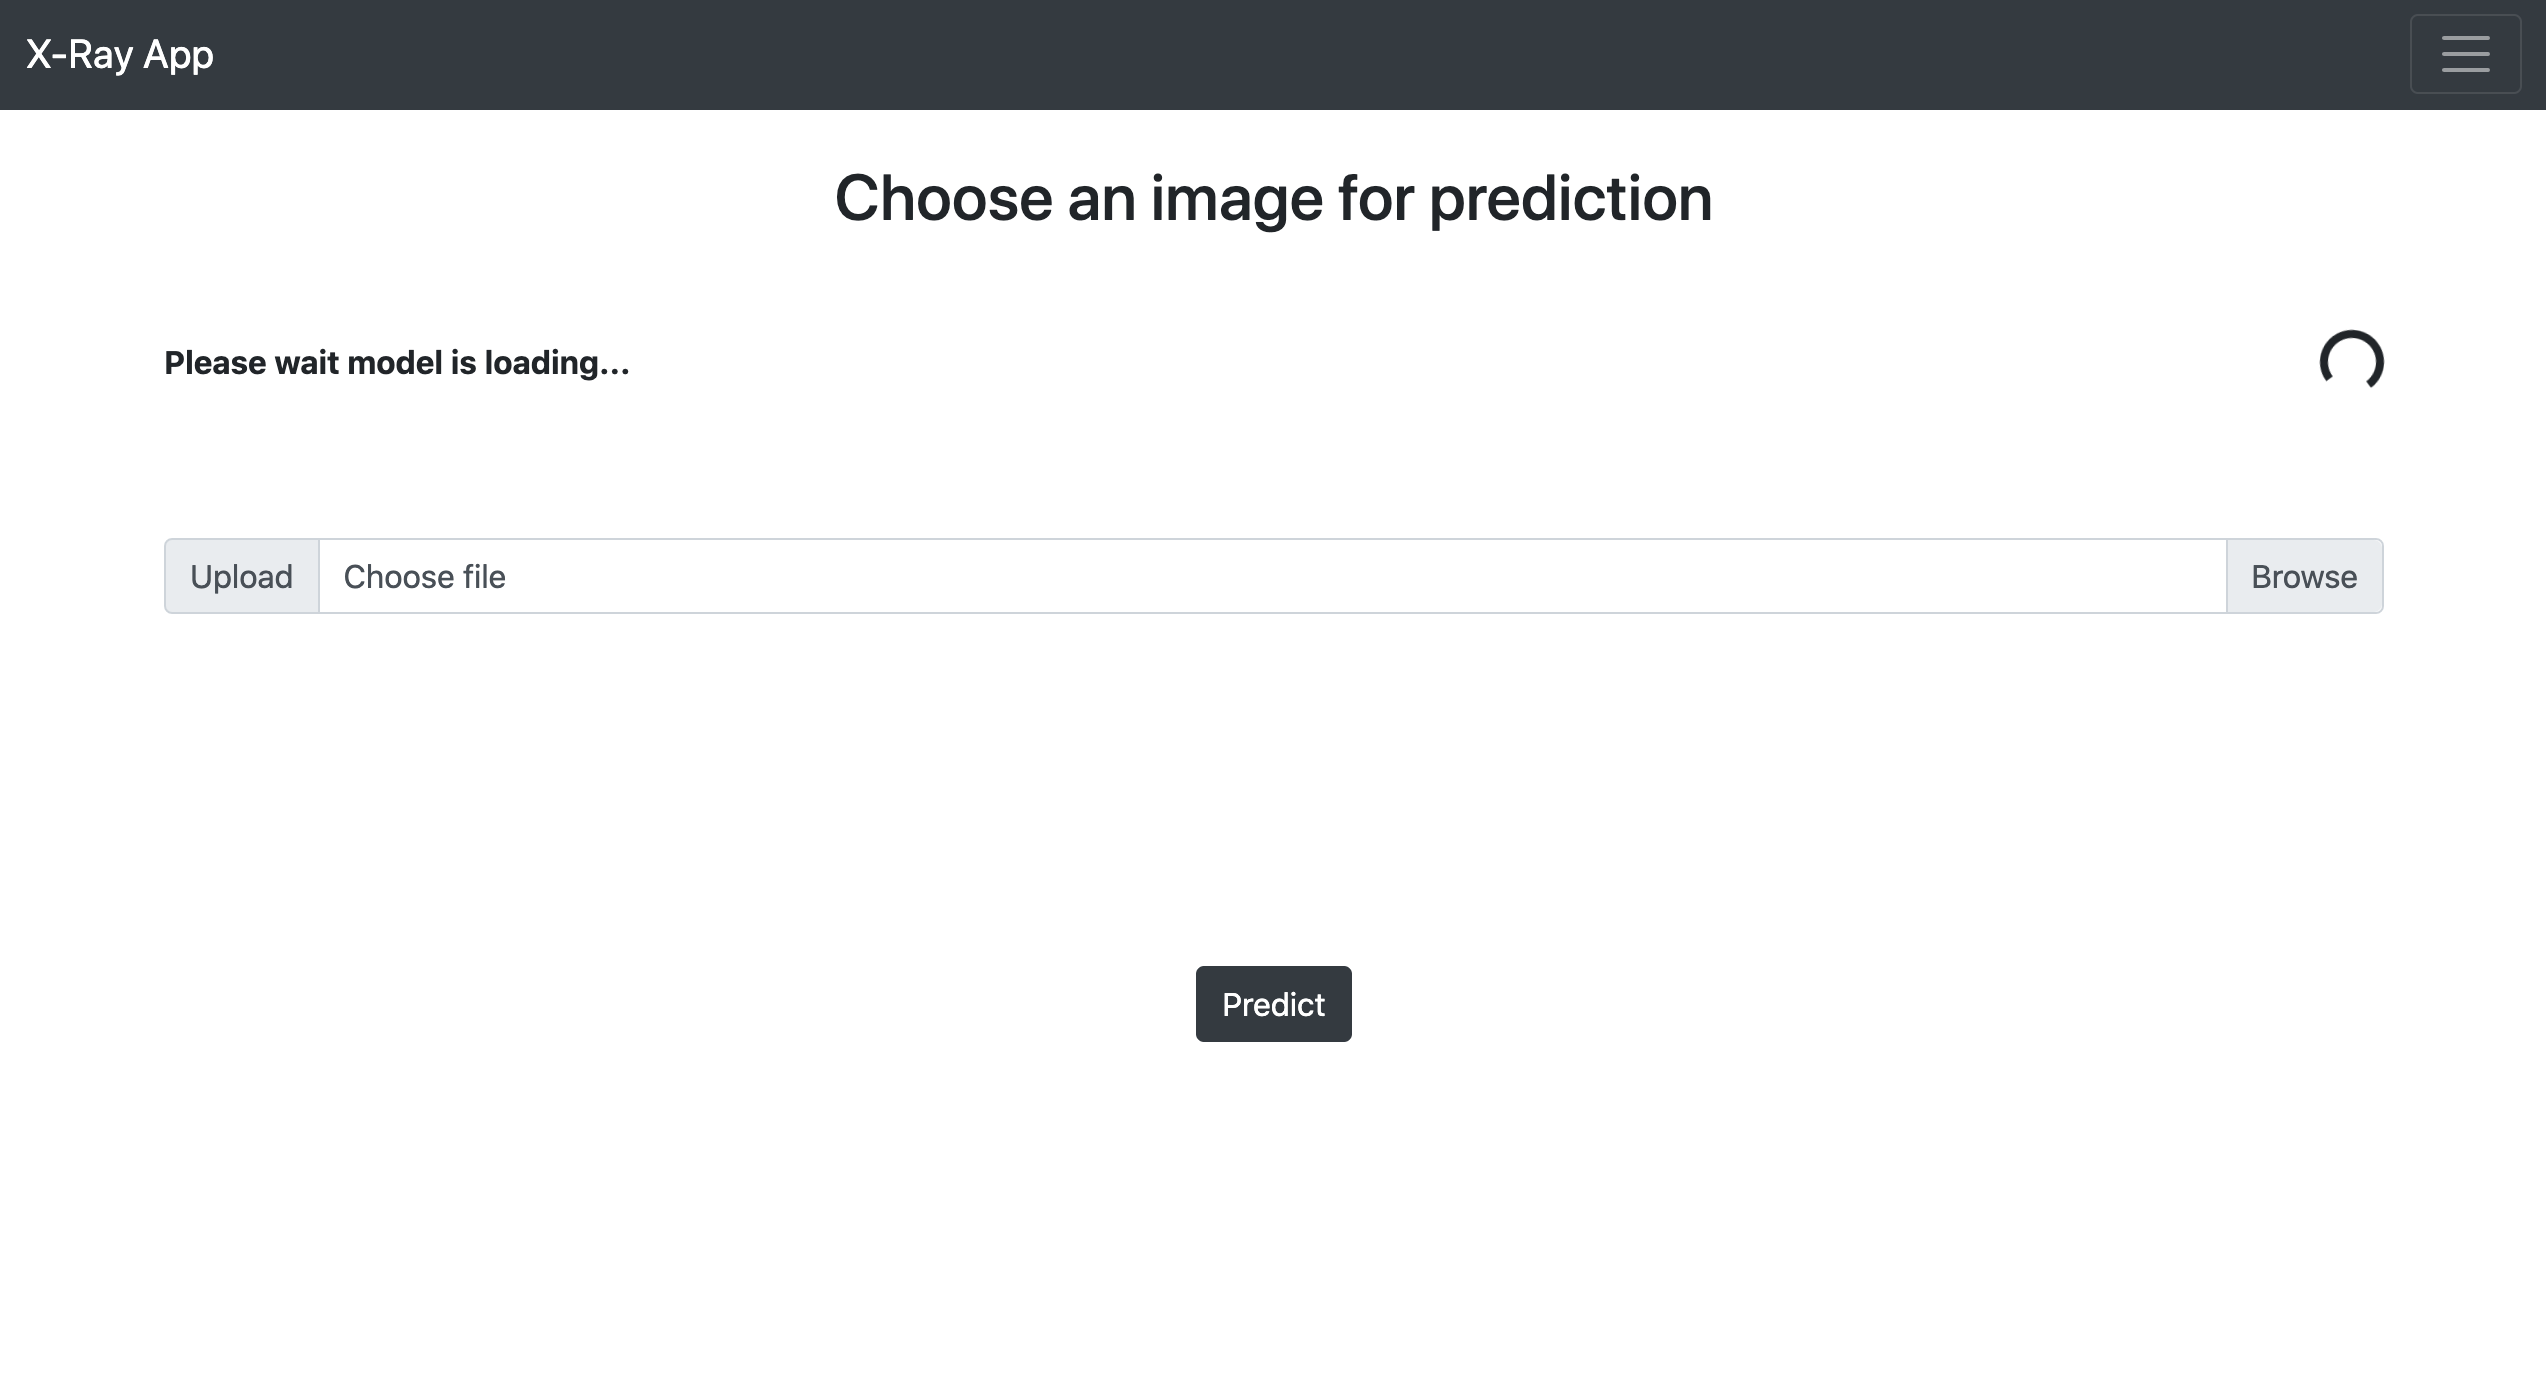
\includegraphics[width=\textwidth]{img/webhome.png}
    \caption{Main page for the deployment.}
    \label{fig:webhome}
\end{figure}

Because loading the model is required step that will take some time, loading of the model is started as soon as the user visiting the website and indicated to the user with spinner containing a message of the load process.
Spinner will be hidden upon completion of the model loading, indication that page ready for prediction.
At this point user can select the X-ray image they want to run predictions which will get loaded to browser to unsure user can verify the image.

\begin{figure}[H]
    \centering
    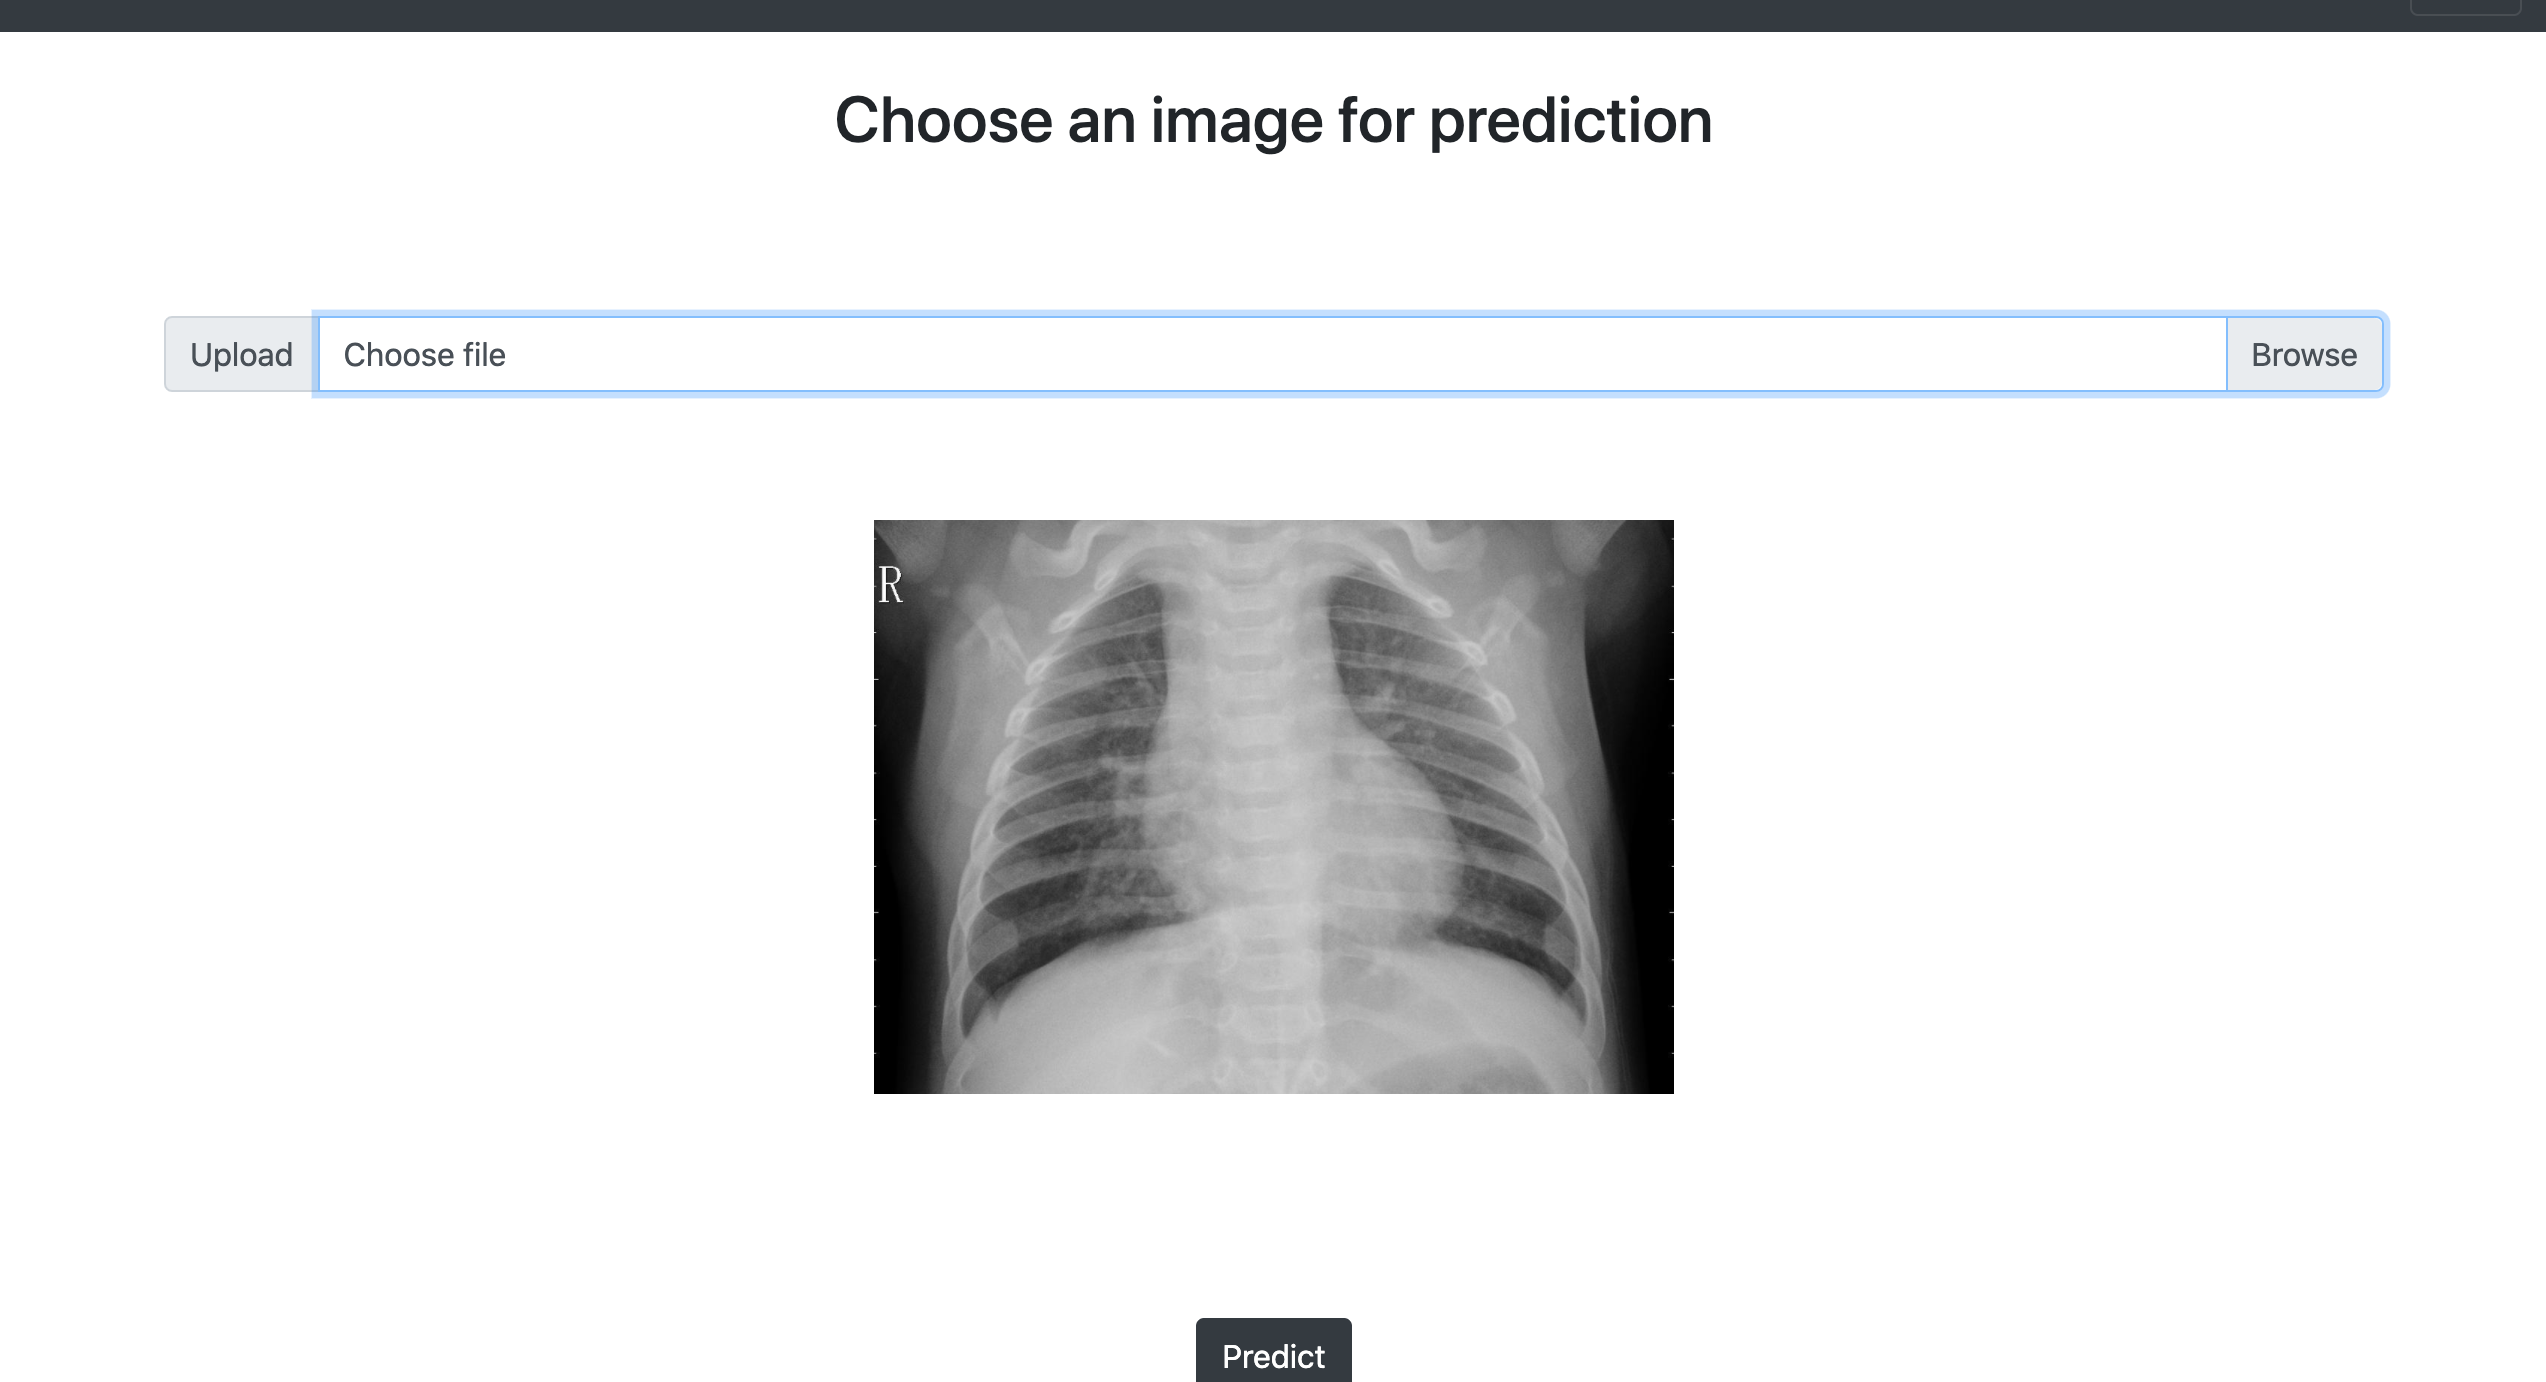
\includegraphics[width=\textwidth]{img/imageloaded.png}
    \caption{X-ray uploaded to website.}
    \label{fig:appimgload}
\end{figure}

At this point user will click predict button and that action will trigger prediction function in JavaScript.
Background JavaScript code fetches the image loaded recently and with the help of build-in function turns image to rank three tensor with RBG channels.
After acquiring the tensor from the image next steps are part of the feature engineering process.
Feature engineering in this app consist of resizing the image to expected dimensions by the model or in other words input shape of the model.
Immediately after that step reshaped image pixels have to be normalize to maximum pixel value that puts tensor values between 0 to 1.
Final, because the original model is trained with batch data input data has to be a rank four tensor rather than three.
Achieving that is possible with a simple step that turning one image to batch data of one incident which commonly referred as expanding the dimensionality.
Now that we have a right shaped tensor, predict method can be called on that image that returns a probability of image having class of \emph{true}, in this case pneumonia.
In the final step this probability will be translated into prediction by checking if the probability is less than or equal to 0.5 then absence of pneumonia will be displayed otherwise prediction will be interpreted as presence of pneumonia.
Product of the prediction then displayed in the web page to the end user along with the probability value as shown below.

\begin{figure}[H]
    \centering
    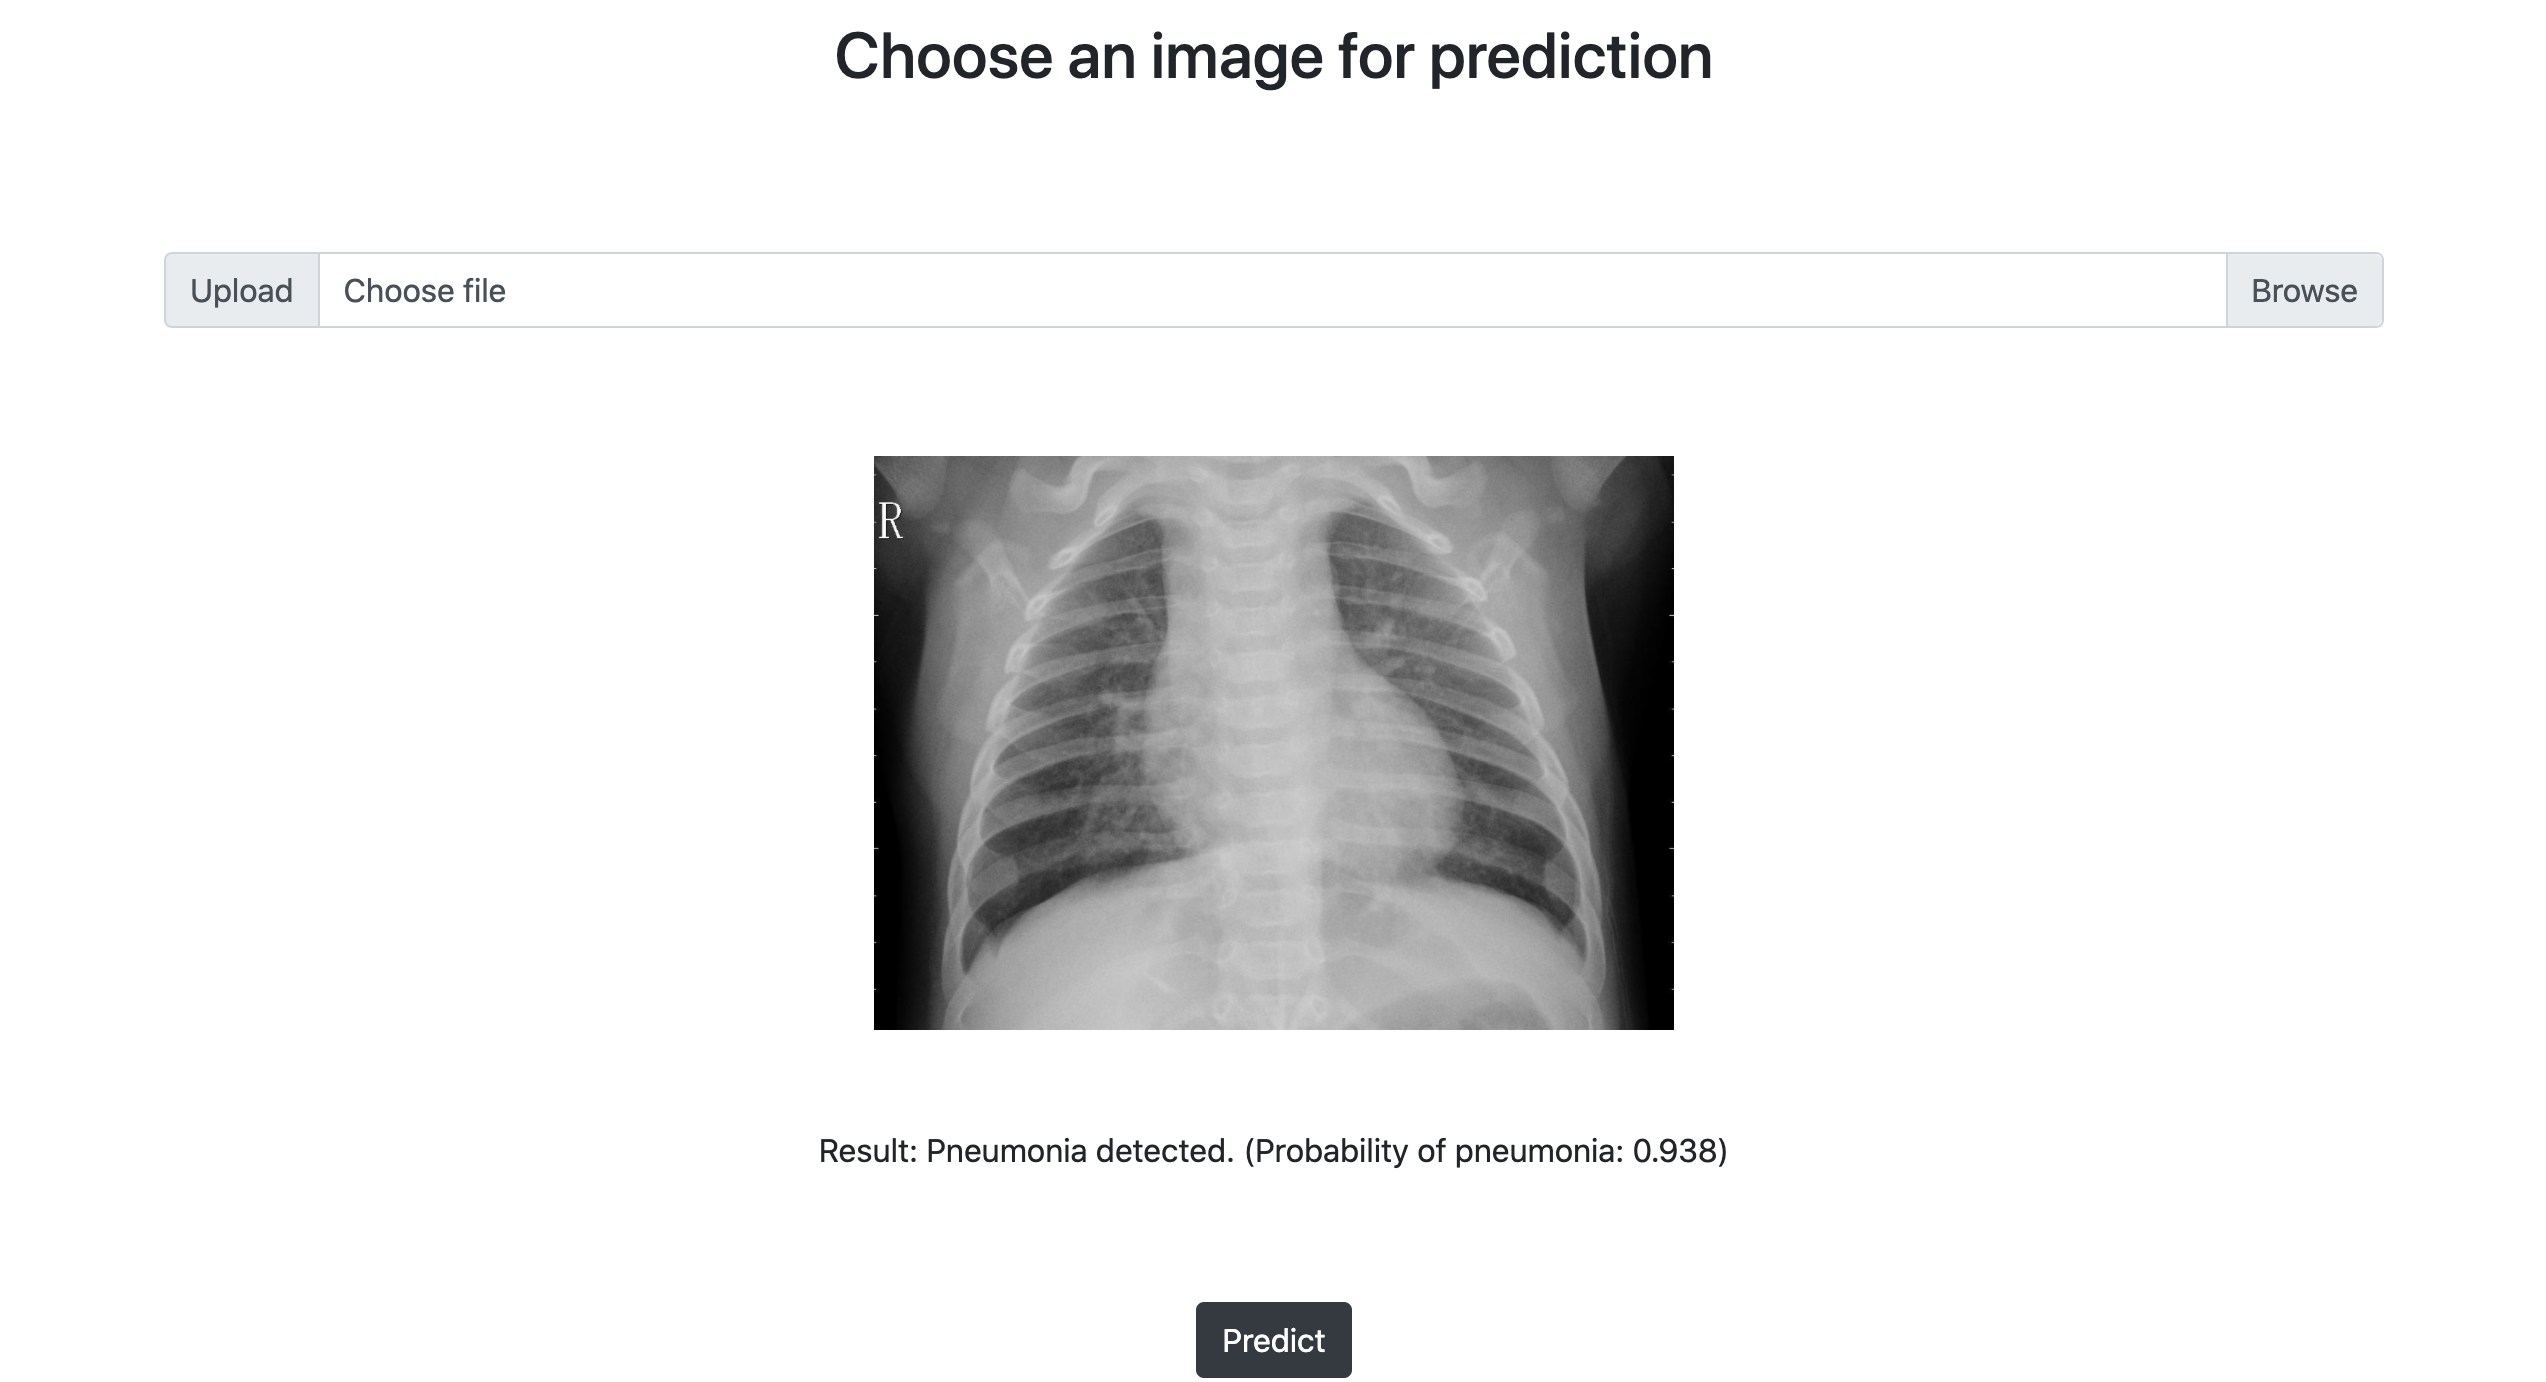
\includegraphics[width=\textwidth]{img/resultimg.png}
    \caption{Prediction results displayed to user.}
    \label{fig:appresult}
\end{figure}

% Why deployment
% why static webpage deployment
% pros of static web page
% - privacy
% - very little or no cost
% cons of static 
% - model is available to anyone
% - loading and processing times long

% Process of implementing my deployment
% webpage is served by GitHub
% image selected by user gets loaded and displayed in page
% Pre-processing
% - turn image to tensor
% - reshape tensor to desired size
% - normalize the tensor values
% - increase input dimension to batch of one

% returns prediction probability
% create a function to predict based on probability